\documentclass[conference]{IEEEtran}
\IEEEoverridecommandlockouts
\usepackage{cite}
\usepackage{amsmath,amssymb,amsfonts}
\usepackage{graphicx}
\usepackage{booktabs}
\usepackage{xcolor}
\usepackage{textcomp}
\newcommand{\E}{\mathbb{E}}
\newcommand{\pb}{p_b}
\setlength{\textfloatsep}{6pt plus 2pt minus 2pt}
\setlength{\floatsep}{6pt plus 2pt minus 2pt}
\setlength{\intextsep}{6pt plus 2pt minus 2pt}
\begin{document}

\title{BMQ: Analytical Modeling of Bursty Multicast Traffic\\in Mesh Networks-on-Chip}

\author{\IEEEauthorblockN{Akshat Sinha}
\IEEEauthorblockA{\textit{CSA, IISc Bengaluru}\\akshatsinha@iisc.ac.in}
\and
\IEEEauthorblockN{Om Gopalkrushna Kumbhare}
\IEEEauthorblockA{\textit{CSA, IISc Bengaluru}\\omgopalkrus1@iisc.ac.in}
\and
\IEEEauthorblockN{Swapnil Aggarwal}
\IEEEauthorblockA{\textit{CiSTUP, IISc Bengaluru}\\swapnila@iisc.ac.in}}

\maketitle

\begin{abstract}
Cache coherence turns a single write or miss into a multicast: one message that must reach many caches, and that completes only when its \emph{last} copy arrives. Most NoCs, including gem5's Garnet, have no multicast hardware; the source network interface (NI) replicates the message and injects the copies one after another through a few virtual channels (VCs). Published analytical models either assume all copies leave in parallel (Moadeli and Vanderbauwhede) or model bursty traffic without multicast (Mandal et~al.). We present BMQ, a queueing model that treats a $K$-way multicast as a batch arriving at the source NI under bursty (generalized geometric) arrivals, computes each copy's departure from the NI's VC and credit rules, and adds a link-wait model for the mesh. Router timing is derived from the pipeline, not fitted. Against gem5/Garnet on SPLASH-4, PARSEC, coherence microbenchmarks and synthetic traffic, BMQ predicts multicast completion latency with 6.4\% mean error on a $4{\times}4$ mesh, against 24.5\% and 34.3\% for the two baselines. At high injection the model is up to 30\% low; we trace this to VCs held at the NI and add a correction that halves the error and finds 9 of 14 saturations instead of 2. On $6{\times}6$ and $8{\times}8$ meshes BMQ stays best (13.4\% and 17.6\%); its error there comes from broadcast-heavy MOESI\_hammer runs.
\end{abstract}

\section{Introduction}
In a many-core chip, coherence traffic is not unicast. A directory protocol sends invalidations to every sharer of a line before a write; a broadcast protocol sends every miss to all other caches~\cite{sorin2011primer}. The action finishes only when the slowest copy arrives, so the quantity that matters is the \emph{completion latency}, the maximum over copies, not the average copy latency.

Garnet~\cite{agarwal2009garnet}, like many NoCs, implements multicast by \emph{source replication}: the NI makes $K$ unicast copies and pushes them through one injection link, limited by $V{=}4$ VCs per virtual network and by credit return. The last of 15 one-flit copies therefore leaves 17 cycles after the first, even on an idle network. On our gem5 traces, multicasts are about 5\% of messages under a broadcast protocol but 42--47\% of network packets.

Two bodies of work come close, and each misses half of this. Moadeli and Vanderbauwhede~\cite{moadeli2009multicast} model multicast but assume the copies leave through parallel ports with Poisson arrivals. Mandal et~al.~\cite{mandal2020bursty} model bursty traffic with generalized geometric (GGeo) arrivals but not multicast, so every copy gets the same mean wait. Real coherence traffic is both: the coefficient of variation of multicast inter-arrival times is far above the Poisson value of 1 (up to 55 for \texttt{fft}).

\textbf{Contributions.} (i)~BMQ, a closed-form model of bursty multicast at the source NI plus mesh link waits, with router timing derived from the pipeline; (ii)~an extended gem5 trace and synthetic traffic setup with a validation pipeline; (iii)~validation on 4$\times$4, 6$\times$6 and 8$\times$8 meshes against both published models re-implemented on the same inputs; (iv)~an analysis of why the model fails at high injection, a derived correction, and its evaluation.

\section{Related Work}
Analytical NoC models mostly address unicast traffic: Ogras and Marculescu model routers as queues~\cite{ogras2007router}, and broadcast models for multicomputers assume Poisson arrivals~\cite{shahrabi2003hypercube}. \textbf{Moadeli and Vanderbauwhede}~\cite{moadeli2009multicast} give the first multicast model for wormhole NoCs (Quarc): channels are M/G/1 queues, a multicast leaves through several injection ports as independent streams, and latency is the expected maximum of exponential waits. \textbf{Mandal et~al.}~\cite{mandal2020bursty,mandal2021wrr} model each router queue as GGeo/G/1~\cite{kouvatsos1994entropy}, propagate burstiness through the network with Whitt-style decomposition~\cite{whitt1983qna}, and fit the burst probability of a real application by replaying its timestamps through a virtual queue. In packet switches, fan-out splitting treats a multicast as batch service~\cite{hui1990multicast}. BMQ combines these: GGeo message arrivals, a $K$-copy batch at one NI, and an exact per-copy schedule from VC allocation (Table~\ref{tab:related}). Without multicast it reduces to the GGeo/D/1 result of Mandal et~al.

\begin{table}[t]
\centering\footnotesize
\caption{Closest analytical models.}\label{tab:related}
\begin{tabular}{@{}lccc@{}}
\toprule
 & Moadeli~\cite{moadeli2009multicast} & Mandal~\cite{mandal2020bursty} & BMQ \\
\midrule
Multicast & yes & no & yes \\
Arrivals & Poisson & GGeo & GGeo \\
Copy injection & parallel ports & independent & one port \\
Wait of copy $j$ & none at source & same for all & depends on $j$ \\
Completion & E[max] exp. & not modeled & max over paths \\
Validated on & own sim. & industrial & gem5 \\
\bottomrule
\end{tabular}
\end{table}

\section{Methodology}
\textbf{Simulation.} We use gem5 v26~\cite{binkert2011gem5} (syscall emulation, X86 \texttt{TimingSimpleCPU}, 2\,GHz) with Ruby and Garnet 3.0, XY routing, 1-cycle routers and links, 4 VCs per virtual network, 1-flit buffers on control vnets and 4-flit on data, 16\,B flits (4\,B in narrow-link runs). Two protocols run in one build: MESI\_Two\_Level (directory) and MOESI\_hammer (broadcast). Meshes are $4{\times}4$ (16 cores), $6{\times}6$ (36 cores, 32 L2/directories) and $8{\times}8$ (64).

\textbf{Trace hook.} We add a hook in Garnet's NI that logs every coherence message \emph{before} replication (creation, first-send and last-VC cycles, source, vnet, flits, fan-out, destinations) and every packet ejection. Latency is measured from the message's estimated arrival at the NI to the ejection of its last copy (completion), or of each copy.

\textbf{Workloads.} Six SPLASH-4~\cite{gomezhernandez2022splash4} kernels (fft, lu-cont, radix, ocean-cont, water-nsquared, barnes) and four PARSEC~\cite{bienia2008parsec} programs (blackscholes, swaptions, fluidanimate, streamcluster) give 10 benchmarks $\times$ 2 protocols = 20 runs per mesh. On $4{\times}4$ we add 42 coherence load-sweep runs from our microbenchmarks (producer-consumer, barrier, lock; 16\,B and 4\,B flits, five load levels). On $4{\times}4$, $6{\times}6$ and $8{\times}8$ we add synthetic runs from an extended Garnet tester with multicast probability, GGeo bursts and a send queue. Measured windows are 50M cycles on $4{\times}4$ and 20M on larger meshes.

\textbf{Model inputs.} BMQ takes traffic parameters, not traces: per-node message rate $\lambda$, multicast fraction $\alpha$, fan-out distribution, packet mix, destination pattern and burst probability $\pb$. For coherence runs we fit them per node from the trace; $\pb$ uses the virtual-queue method of Mandal et~al.\ in closed form (Lindley recursion on a unit-service queue). Router constants are \emph{derived}, never fitted (Sec.~\ref{sec:timing}). For synthetic runs the inputs are the gem5 command-line settings; nothing is fitted.

\textbf{Baselines.} We re-implemented both published models on BMQ's own inputs, mesh and derived zero-load timing, so only the queueing model differs. Mandal: per-copy GGeo/G/1 queues with departure-SCV propagation. Moadeli: M/G/1 channels with backward service times and an expected maximum of exponentials.

\section{Analytical Model}
\label{sec:model}
\textbf{Setting.} Time is slotted (one cycle). A link carries one flit per cycle; a packet has $L$ flits. Each node has one NI feeding one router; XY routing. A message is a unicast ($K{=}1$, probability $1{-}\alpha$) or a $K$-way multicast. The NI keeps one FIFO queue per (node, vnet). The latency of a copy is built from four terms: the wait for the NI queue, the copy's own departure time from the NI, link waits, and the zero-load trip.



\subsection{Bursty arrivals}
In GGeo, after a message the next arrives in the \emph{same cycle} with probability $\pb$, otherwise after a geometric gap. Counted per cycle, a cycle has arrivals with probability $\sigma$ and then brings $G\sim\mathrm{Geom}(1{-}\pb)$ messages, $\E[G]=1/(1{-}\pb)$. Matching the rate $\lambda$ gives $\sigma=\lambda(1{-}\pb)$. With $N$ the number of messages in a cycle,
\begin{equation}
\E[N]=\lambda,\qquad \E[N(N{-}1)]=\frac{2\lambda\pb}{1-\pb}.
\label{eq:N}
\end{equation}
$N(N{-}1)$ counts ordered pairs of messages that share a cycle. Waiting needs two requests for the server at once, so this is the raw measure of collisions from burstiness; it is 0 when $\pb{=}0$.

\subsection{The copy schedule at the source NI}
A copy needs one of the $V$ VCs of its vnet. The link sends one flit per cycle, each flit needs a downstream credit, and a VC is free again $R$ cycles after its copy's tail flit is sent ($R{=}5$ from the pipeline, Sec.~\ref{sec:timing}). Let $a_j$ be the cycle copy $j$ obtains a VC and $s_j$ the cycle it is sent, from the first copy. For one-flit copies
\begin{equation}
a_j=\begin{cases}0 & j\le V\\ s_{j-V}+R & j>V\end{cases},\qquad s_j=\max(a_j,\,s_{j-1}+1).
\label{eq:sched}
\end{equation}
For longer packets the same rules apply flit by flit with credits (function \texttt{ni\_schedule}). Let $\tau_j$ be the cycle copy $j$'s tail leaves, counted from the first flit. For $K{=}15$, $L{=}1$: $s=0,1,2,3,\,5,6,7,8,\,10,11,12,13,\,15,16,17$ (Fig.~\ref{fig:sched}): four copies go at once, then a pause for VCs. This reproduces Garnet's measured last-copy time for every $K$ and for 2-flit packets. The multicast keeps the NI queue busy for $B(K,L)=\tau_K+1$ cycles; a unicast for $B=L$.

\begin{figure}[t]
\centering
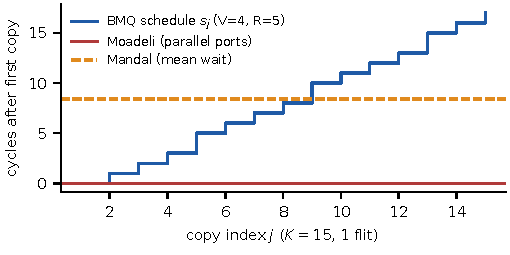
\includegraphics[width=.9\columnwidth]{figs/f_schedule.pdf}
\caption{Departure of the 15 copies of a broadcast from an idle NI. Moadeli assumes all leave at 0; Mandal assigns every copy the mean.}
\label{fig:sched}
\end{figure}

\subsection{Waiting in the NI queue}
Let $A=B_1+\dots+B_N$ be the work arriving in a cycle. Conditioning on $N$,
\begin{align}
\rho&=\E[A]=\lambda\,\E[B],\nonumber\\
\E[A(A{-}1)]&=\lambda(\E[B^2]-\E[B])+\E[N(N{-}1)]\,\E[B]^2.
\label{eq:A}
\end{align}
The two terms name the two causes of waiting: a single message bringing many cycles of work (a multicast) and several messages arriving together (a burst). Let $U$ be the backlog at the start of a cycle. The queue obeys $U'=U+A-1+\mathbf 1\{U+A=0\}$. Taking the mean gives $P(U{+}A{=}0)=1{-}\rho$; squaring and taking the mean gives, in the standard discrete-time way~\cite{bruneel1993discrete},
\begin{equation}
\E[U]=\frac{\E[A(A{-}1)]}{2(1-\rho)}.
\label{eq:U}
\end{equation}
A message also waits for those of its own cycle served first: it shares its cycle with $2\pb/(1{-}\pb)$ others on average, each ahead with probability $\tfrac12$. The wait of its \emph{first copy} is
\begin{equation}
W_{\rm head}=\E[U]+\frac{\pb\,\E[B]}{1-\pb}.
\label{eq:Whead}
\end{equation}
Copy $j$ then leaves $\tau_j$ cycles later. The model is stable only for $\rho<1$, and the $1/(1{-}\rho)$ factor makes waits explode near saturation.

\subsection{Waiting at links}
Walk every flow (unicast flows and the copy flows) along its XY path and record, for each link $\ell$, the packet rate $\lambda_i$ entering through each input port $i$. With $\lambda_\ell=\sum_i\lambda_i$, mean packet length $T_\ell$, length SCV $C_{S,\ell}^2$, and $\rho_\ell=\lambda_\ell T_\ell$:
\begin{equation}
W_\ell=(1-h_\ell)\,\frac{\rho_\ell T_\ell(1+C_{S,\ell}^2)}{2(1-\rho_\ell)},\qquad h_\ell=\frac{\sum_i\lambda_i^2}{(\sum_i\lambda_i)^2}.
\label{eq:link}
\end{equation}
The second factor is the Pollaczek--Khinchine wait. $h_\ell$ is the probability that two packets on $\ell$ came through the same port; such packets arrive in single file and cannot collide, so $1{-}h_\ell$ (the \emph{merge factor}) keeps only the collidable pairs. A link fed by one port never queues. For one-flit packets (\ref{eq:link}) is exactly the Karol--Hluchyj--Morgan result~\cite{karol1987input}, $W=[(\sum\lambda_i)^2-\sum\lambda_i^2]/(2\rho(1-\rho))$. Each link uses only its own rates, so there is no iteration.

\subsection{Latency and completion; derived router timing}
\label{sec:timing}
Copy $j$ of a multicast to destinations $d_1,\dots,d_K$ (hop count $H_j$) has latency, and the multicast completes with its slowest copy:
\begin{equation}
T_j=W_{\rm head}+\tau_j+\!\!\sum_{\ell\in{\rm path}_j}\!\!W_\ell+T_{\rm hop}(H_j),\qquad C=\max_j T_j.
\label{eq:T}
\end{equation}
A unicast is the case $K{=}1$ with its own $\tau(L)$. All constants follow from Garnet's pipeline (NI stage, one-stage router, one-cycle links, credits applied the cycle after they arrive): $T_{\rm hop}(H)=t_{NI}+(H{+}1)t_{r}+(H{+}2)t_{\ell}=4+2H$ and $R=t_{NI}+t_r+2t_\ell+1=5$. They match Garnet's minimum measured latency exactly for 1-flit, 5-flit (4-flit buffers), 5-flit (1-flit buffers, $24{+}2H$) and 4\,B-flit packets at every hop count 0--6.

\textbf{Assumptions.} Arrivals at a link are random, because a link's inputs are other links delivering at most one flit per cycle; waits are averages (a max of means slightly underestimates the mean of the max); buffers are infinite; and the NI queue starts every multicast with all VCs free. Sec.~\ref{sec:high} shows the last two matter near saturation.

\section{Results}
All errors compare a model's multicast completion latency with Garnet's, as $|{\rm pred}-{\rm meas}|/{\rm meas}$ averaged over runs that Garnet does not saturate (unicast latency for unicast runs). A model that calls a run saturated when Garnet does not has a \emph{false saturation}; such runs are not in the mean. This section uses the model of Sec.~\ref{sec:model} (no correction), on $4{\times}4$. We first test it on real coherence traffic, where loads are light, and then on synthetic traffic driven up to saturation.

\subsection{Coherence traffic: standard benchmarks and load sweeps}
\begin{table}[t]
\centering\footnotesize
\caption{$4{\times}4$ coherence runs: mean $|$error$|$ (\%) of completion (false saturations in brackets).}
\label{tab:main}
\begin{tabular}{@{}lrrrr@{}}
\toprule
Workload (runs) & BMQ & Mandal & Moadeli & Moad.\ med.\\
\midrule
Standard benchmarks (20)    & \textbf{6.4} & 24.5 & 34.3 (1) & 27.3\\
Coherence sweep 16\,B (30)  & \textbf{8.2} & 22.8 & 223 (11) & 26.4\\
Coherence sweep 4\,B (12)   & \textbf{11.3} & 28.0 & 46.5 (3) & 36.3\\
\bottomrule
\end{tabular}
\end{table}

\begin{figure*}[t]
\centering
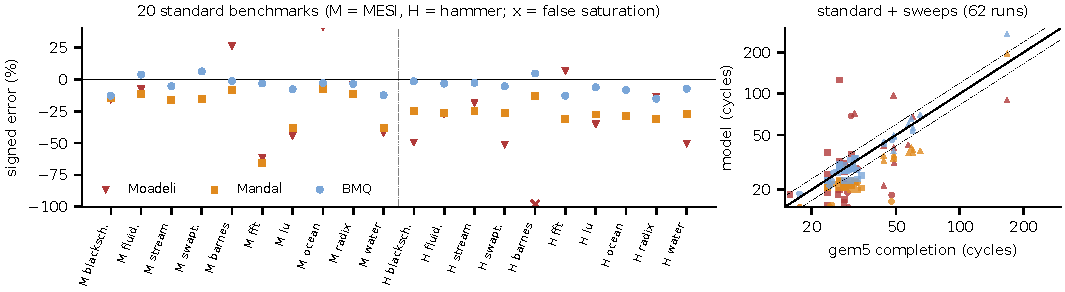
\includegraphics[width=\textwidth]{figs/f_coh.pdf}
\caption{$4{\times}4$ coherence traffic. Left: signed error of each of the 20 standard benchmarks. Right: predicted vs.\ measured completion for standard benchmarks ($\circ$), 16\,B sweep ($\square$) and 4\,B sweep ($\triangle$); dotted lines are $\pm20\%$.}
\label{fig:coh}
\end{figure*}

\textbf{Standard benchmarks.} BMQ's mean error is 6.4\% (median 5.4\%); Mandal's is 24.5\% and Moadeli's 34.3\%, with one false saturation (Table~\ref{tab:main}, Fig.~\ref{fig:coh} left). BMQ is within 15.3\% on every run and slightly low on most (signed $-4.9\%$): it ignores router-internal effects and the spread of waits. The worst runs are hammer \texttt{radix} ($-15.2\%$), MESI \texttt{blackscholes} ($-12.9\%$), hammer \texttt{fft} ($-12.8\%$) and MESI \texttt{water-nsquared} ($-12.4\%$). Peak link utilization is under 0.10 here, so nearly all of the gap to the baselines is at the NI: the schedule~(\ref{eq:sched}) applies even at zero load. Example: for a 1-flit broadcast to 15 caches from an idle NI, Garnet's last copy arrives after 29.2 cycles; BMQ predicts 27.6, Mandal 21.3 and Moadeli 14.1.

\textbf{Coherence load sweep.} Over 42 runs (two protocols, two flit widths, three kernels, five loads) BMQ's error is 8.2\% (16\,B flits) and 11.3\% (4\,B flits), against 22.8\% and 28.0\% for Mandal. In Fig.~\ref{fig:coh} (right) BMQ follows the diagonal over a decade of latencies while Mandal sits below it, the gap growing with $K$. Moadeli errs in both directions: too low at light load (parallel ports) and too high under load, where its blocking recursion charges each channel for the whole trip, which does not fit pipelined VC routers. It falsely saturates 14 of the 42 runs, so its mean (223\% on the 16\,B sweep) is dominated by those runs and its median (26\%) is the fairer summary. BMQ's largest errors are two known failure modes: MESI lock kernels ($-9$ to $-28\%$), where a multicast is followed by correlated data packets and the next multicast finds VCs still busy, and hammer 4\,B lock with no spin ($+62\%$), where lock hand-offs are self-paced so arrivals depend on the network, against the open-loop assumption.

\subsection{Synthetic traffic: high link load and saturation}
\begin{table}[t]
\centering\footnotesize
\caption{$4{\times}4$ synthetic runs: mean $|$error$|$ (\%) on runs Garnet does not saturate, and saturations predicted ($^\dagger$BMQ/Mandal/Moadeli).}
\label{tab:synth}
\begin{tabular}{@{}lrrrr@{}}
\toprule
Workload & BMQ & Mandal & Moadeli & Sat.\ found\\
\midrule
Unicast (25 + 5 sat.) & \textbf{2.5} & 12.7 & 108 (20 false) & 5/5/5 of 5$^\dagger$\\
Multicast (17 + 14 sat.) & \textbf{12.5} & 60.4 & 14 of 17 false & 2/2/14 of 14$^\dagger$\\
\bottomrule
\end{tabular}
\end{table}

\begin{figure*}[t]
\centering
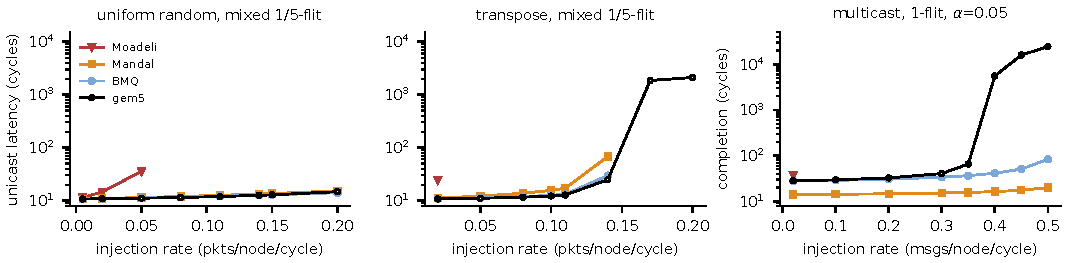
\includegraphics[width=\textwidth]{figs/f_synth.pdf}
\caption{$4{\times}4$ synthetic traffic up to saturation (log scale; a model line stops where it predicts saturation). Left, centre: unicast latency, uniform-random and transpose, mixed 1-/5-flit packets. Right: multicast completion, configuration~A (1-flit, 5\% broadcasts to 15 caches). Garnet saturates at 0.40 in the right panel; Moadeli stops at the first point.}
\label{fig:synth}
\end{figure*}

\textbf{Unicast: the link model at high load.} With $K{=}1$ the NI term vanishes and the runs test the link formula~(\ref{eq:link}). Peak link utilization reaches 0.97 (uniform random and transpose, 1-flit and mixed packets). BMQ has 2.5\% error on the 25 unsaturated runs, with all five runs that saturate in Garnet predicted saturated (Fig.~\ref{fig:synth}, left and centre), and Mandal 12.7\%. On mixed transpose traffic the merge factor correctly gives no wait on single-input links, where a $C_S^2$-based model predicts congestion. The remaining gap (about 8\% low at $\rho_\ell{=}0.5$) is router-internal contention (switch allocation, head-of-line blocking). Moadeli's wormhole blocking recursion saturates 20 of the 25 runs that Garnet does not.

\textbf{Multicast: where the model fails.} With bursty multicast at the NI the picture changes. Over 17 unsaturated runs the error is 12.5\%, and the model is low on every run (Fig.~\ref{fig:synth}, right): at light load it follows Garnet, but past rate 0.2 it falls behind, and it does not saturate when Garnet does. Of 14 runs where Garnet saturates, BMQ predicts saturation in 2, Mandal in 2, while Moadeli predicts saturation everywhere (14 of 14) and also in 14 of the 17 runs that do not saturate. Section~\ref{sec:high} analyses this failure and corrects it.

\section{Why the Model Breaks at High Load}
\label{sec:high}
\begin{figure*}[t]
\centering
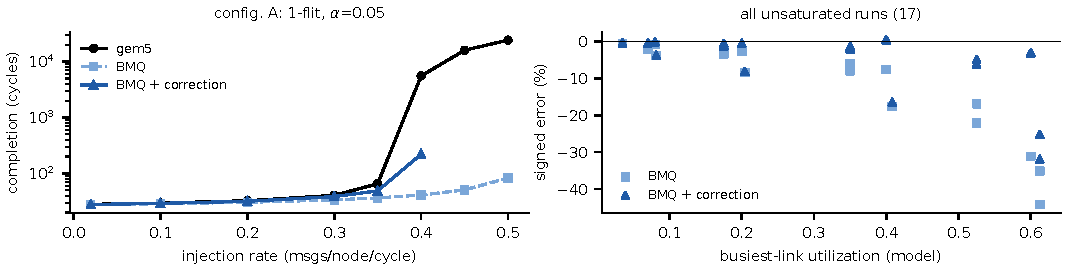
\includegraphics[width=\textwidth]{figs/f_highload.pdf}
\caption{High-injection multicast on $4{\times}4$. Left: completion vs.\ rate (config.\ A: 1-flit packets, 5\% broadcasts); gem5 saturates at 0.40, the uncorrected model is flat and low. Right: signed error of all 17 unsaturated runs vs.\ busiest-link utilization.}
\label{fig:highload}
\end{figure*}
We drove the NI, schedule and links up to saturation with four open-loop configurations (A: 1-flit, $\alpha{=}0.05$; B: $\alpha{=}0.2$; C: bursty $\pb{=}0.5$; D: mixed 1- and 5-flit; rates 0.02--0.5 msgs/node/cycle, every multicast a 15-way broadcast). Model inputs are the gem5 settings. On the 17 unsaturated runs the mean error is 12.5\% and the model is \emph{low on every run}: 3.0\% for busiest-link utilization below 0.25, 9.8\% at 0.25--0.45 and 29.9\% at 0.45--0.65 (Fig.~\ref{fig:highload}). It also misses saturation: Garnet saturates in 14 runs at about 70\% of the model's saturating utilization, and the model predicts only 2. Unicast-only traffic did not show this (Garnet saturated where the model did), so the cause is specific to the NI.

\textbf{Locating the gap.} The time until a message's last copy obtains its VC (measured before the network) is under-predicted by as much as completion, so the missing time is waiting at the source NI. Replaying the NI trace with Garnet's NI rules reproduces gem5 only when VCs are held about 0.7 cycles longer than $R$, which points to downstream waits. Three resources are modeled as unlimited:
\begin{enumerate}
\item \textbf{NI VCs between messages.} A VC is held for $R{=}5$ cycles after its tail leaves, so with $V{=}4$ an NI can start at most $V/R=0.8$ packets per cycle, not 1. The schedule (\ref{eq:sched}) applies this limit within one multicast, but the queue assumes every new message finds all VCs free.
\item \textbf{The shared injection link.} A node's vnets share one link into the router; the model gives each vnet its own queue and link (configuration D).
\item \textbf{Finite router buffers.} Waiting room is infinite in (\ref{eq:link}); Garnet's 1- and 4-flit buffers back-pressure the NI once downstream VCs are held.
\end{enumerate}

\textbf{The correction.} All three are added, derived from the pipeline and with no fitted constants:
\begin{enumerate}
\item \emph{NI service limited by VCs.} A message holds VCs for $H=\sum_j(\tau_j+R-a_j)+K D$ VC-cycles, where $D$ is the mean wait of the queue's copies at the injection link and first router. The service time becomes
\begin{equation}
B_{\rm eff}=\max(B,\ H/V),
\label{eq:Beff}
\end{equation}
and replaces $B$ in (\ref{eq:A})--(\ref{eq:Whead}). A 1-flit unicast now costs $5/4$ cycles (NI capacity 0.8); a 15-way broadcast $18.75$ instead of $18$.
\item \emph{Injection link as a channel.} It is treated like a mesh link in (\ref{eq:link}) with the node's vnets as input ports, and a node saturates when its total injection load reaches 1.
\item \emph{Downstream VC wait.} A packet crossing channel $c$ needs one of the $V$ VCs of its vnet at the next router and holds it for $S=L-1+R_c+D_{\rm next}$ cycles ($R_{\rm link}{=}3$, $R_{\rm eject}{=}2$ from the pipeline). Each (channel, vnet) is an M/D/$V$ pool:
\begin{equation}
W_{\rm vc}=(1-h)\,\frac{\mathcal C(V,a)\,S}{2\,(V-a)},\qquad a=\lambda S,
\label{eq:vc}
\end{equation}
with $\mathcal C$ the Erlang-C probability that all $V$ VCs are busy. $D_{\rm next}$ depends on downstream waits, so (\ref{eq:vc}) is iterated backward from $D{=}0$; a channel with $a\ge V$ saturates. $W_{\rm vc}$ is added to each link term of (\ref{eq:T}).
\end{enumerate}
With all three off the model is exactly Sec.~\ref{sec:model}.

\begin{table}[t]
\centering\footnotesize
\caption{Effect of the correction on the 17 unsaturated and 14 saturated synthetic multicast runs ($4{\times}4$).}
\label{tab:corr}
\begin{tabular}{@{}lrrr@{}}
\toprule
Busiest-link utilization & Runs & BMQ & + correction \\
\midrule
below 0.25 & 8 & 3.0 & 1.9 \\
0.25--0.45 & 4 & 9.8 & 5.1 \\
0.45--0.65 & 5 & 29.9 & 14.3 \\
\textbf{All unsaturated} & 17 & \textbf{12.5} & \textbf{6.3} \\
Saturations found (of 14) & 14 & 2 & 9 \\
\bottomrule
\end{tabular}
\end{table}

\textbf{Results with the correction.} On the 17 unsaturated runs the mean error falls from 12.5\% to 6.3\% (median 2.1\%): from 3.0\% to 1.9\% below utilization 0.25, from 9.8\% to 5.1\% at 0.25--0.45 and from 29.9\% to 14.3\% at 0.45--0.65. Predicted saturations rise from 2 to 9 of 14, with no false saturation (Fig.~\ref{fig:highload}). The shared injection link matters in configuration D, where the VC term alone did not help. The correction is inert at light load: on the standard benchmarks the error is 6.4\% either way, and on the 16\,B sweep 8.2\% vs.\ 8.4\%. It does not fix the MESI lock runs ($-23.5\%$ to $-22.6\%$): the data burst accompanying an invalidation is correlated with it, which average injection-link load cannot capture.

\section{Correction Across Mesh Sizes}
\begin{figure*}[t]
\centering
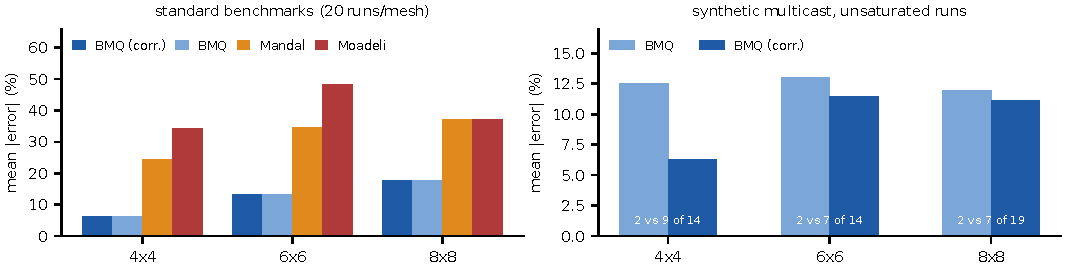
\includegraphics[width=\textwidth]{figs/f_meshes.pdf}
\caption{Left: standard benchmarks, mean error of the four models on three mesh sizes (Moadeli omits its false saturations: 1, 4 and 10 runs). Right: synthetic multicast, BMQ without and with the correction; labels give saturations caught of those that gem5 shows (uncorrected vs.\ corrected).}
\label{fig:meshes}
\end{figure*}
We repeat the comparison on $6{\times}6$ and $8{\times}8$ with the same models and inputs. Coherence runs use the 10 standard benchmarks under both protocols (20 per mesh, 20M-cycle window; one $8{\times}8$ hammer run, \texttt{ocean-cont}, hit our 6\,h limit and is measured over 14.9M cycles), SPLASH-4 uses 32 threads on $6{\times}6$, and synthetic rates are scaled so the busiest queue has the same utilization as on $4{\times}4$; broadcasts are 31--35 or 63 copies.

\begin{table}[t]
\centering\small
\caption{Standard benchmarks: mean $|$error$|$ (\%) of completion by mesh and protocol (20 runs per mesh).}
\label{tab:mesh}
\begin{tabular}{@{}llrrr@{}}
\toprule
Mesh & Protocol & BMQ & Mandal & Moadeli \\
\midrule
$4{\times}4$ & MESI & \textbf{5.9} & 22.7 & 27.5 \\
 & hammer & \textbf{6.8} & 26.3 & 41.9 \\
$6{\times}6$ & MESI & \textbf{2.9} & 25.0 & 45.2 \\
 & hammer & \textbf{23.9} & 44.1 & 53.4 \\
$8{\times}8$ & MESI & \textbf{7.0} & 19.3 & 33.0 \\
 & hammer & \textbf{28.3} & 55.2 & 53.2 \\
\bottomrule
\end{tabular}
\end{table}

\textbf{Standard benchmarks.} BMQ is the most accurate model on every mesh, by 2--4$\times$ over Mandal (Fig.~\ref{fig:meshes}): 6.4\%, 13.4\% and 17.6\% against Mandal's 24.5\%, 34.5\% and 37.3\%, and Moadeli's 34.3\%, 48.2\% and 37.1\% (with 1, 4 and 10 false saturations, so that the last number is flattered by the runs it drops). BMQ never falsely saturates on coherence traffic. Error grows with mesh size and is almost all underprediction (signed $-4.8$, $-12.2$, $-16.6\%$). Table~\ref{tab:mesh} shows where it comes from: MESI stays at 3--7\% on every mesh, since its multicasts are invalidations to the current sharers (a few copies), while MOESI\_hammer, whose every miss broadcasts to all 15, 35 or 63 other caches, grows from 6.8\% to 23.9\% and 28.3\%.

\textbf{Why hammer degrades.} On most hammer runs BMQ is still within 10--25\%, but a few benchmarks are far below Garnet (6$\times$6 \texttt{radix}: $-64\%$, 159 cycles vs.\ 58; 8$\times$8 \texttt{water-nsquared}: $-77\%$, 414 vs.\ 97). The correction does not fire on these runs (same error with it off), so the model sees light average load. A trace analysis finds that its \emph{mechanics} are right and its \emph{inputs}, averages over a 20M-cycle window, are not. First, broadcast arrives in trains at home NIs, with gaps of 3--20 cycles against 45 or 80 cycles of NI service per broadcast on $6{\times}6$ and $8{\times}8$; $\pb$ fitted at a one-cycle scale is 0 and cannot see them. Second, overload phases: in 8$\times$8 \texttt{water-nsquared} the first 1M cycles carry 33\% of broadcasts at about 1030 cycles completion, while the rest is at 96--115 cycles against BMQ's 96.5. In its quietest 1M-cycle window BMQ is within 11\% on 16 of 20 hammer runs.

\textbf{Synthetic traffic.} The correction keeps helping where it was designed to, but by less on larger meshes (Fig.~\ref{fig:meshes}, right): error 12.5\%$\to$6.3\% ($4{\times}4$), 13.0\%$\to$11.4\% ($6{\times}6$), 11.9\%$\to$11.1\% ($8{\times}8$); saturations caught 2$\to$9 of 14, 2$\to$7 of 14 and 2$\to$7 of 19, with no false alarm. Mandal (60--78\%) and Moadeli (every $8{\times}8$ run false) are far behind. Synthetic unicast stays at 1.1\% ($6{\times}6$) and 1.0\% ($8{\times}8$), against 3.4\% and 11.5\% for Mandal.

\textbf{What we did not adopt.} Fitting $\pb$ at the NI service timescale lowered hammer error ($4{\times}4$: 6.8\%$\to$3.8\%; $6{\times}6$: 23.9\%$\to$15.4\%) but raised the 4\,B sweep error from 11.3\% to 23.9\%. A per-window fit that flags overloaded windows is future work.

\section{Conclusion and Future Work}
BMQ models the one thing that sets multicast apart in a replicating NoC: the copies of a message leave the source one after another under VC and credit rules. Combined with GGeo arrivals, a batch queue at the NI and a merge-factor link wait, with router timing derived rather than fitted, it predicts completion latency within 6.4\% (mean) on a $4{\times}4$ mesh, $2$--$4\times$ better than the two published models, and unicast latency within 1--3\% on synthetic traffic. Its main failure at high injection is the NI: VCs are held between messages. A correction derived from the pipeline halves the error there (12.5\%$\to$6.3\%) and finds 9 of 14 saturations, without affecting the light-load results. On larger meshes BMQ remains the best model (13.4\% and 17.6\%); the residual error is concentrated in broadcast-heavy MOESI\_hammer, whose traffic is uneven in time. Validation is on Garnet only.

\textbf{Future work.} (1) Per-window fitting and prediction for time-varying broadcast traffic. (2) Carrying VC state from one multicast to the next, for lock-like closely spaced multicasts. (3) Finite-buffer backpressure beyond the M/D/$V$ term. (4) Checking the model's design-space predictions (copy order, VC count) in gem5. (5) A second simulator such as BookSim, to test that BMQ is not Garnet-specific.

\begin{thebibliography}{99}
\footnotesize
\bibitem{sorin2011primer} D.~J. Sorin, M.~D. Hill, and D.~A. Wood, \emph{A Primer on Memory Consistency and Cache Coherence}. Morgan \& Claypool, 2011.
\bibitem{agarwal2009garnet} N.~Agarwal, T.~Krishna, L.-S. Peh, and N.~K. Jha, ``GARNET: A detailed on-chip network model inside a full-system simulator,'' in \emph{Proc. IEEE ISPASS}, 2009.
\bibitem{binkert2011gem5} N.~Binkert \emph{et al.}, ``The gem5 simulator,'' \emph{SIGARCH Comput. Archit. News}, vol.~39, no.~2, pp.~1--7, 2011.
\bibitem{gomezhernandez2022splash4} E.~J. G\'omez-Hern\'andez \emph{et al.}, ``Splash-4: A modern benchmark suite with lock-free constructs,'' in \emph{Proc. IEEE IISWC}, 2022.
\bibitem{bienia2008parsec} C.~Bienia, S.~Kumar, J.~P. Singh, and K.~Li, ``The PARSEC benchmark suite: Characterization and architectural implications,'' in \emph{Proc. PACT}, 2008.
\bibitem{ogras2007router} U.~Y. Ogras and R.~Marculescu, ``Analytical router modeling for networks-on-chip performance analysis,'' in \emph{Proc. DATE}, 2007.
\bibitem{shahrabi2003hypercube} A.~Shahrabi, L.~M. Mackenzie, and M.~Ould-Khaoua, ``An analytical model of wormhole-routed hypercubes under broadcast traffic,'' \emph{Perform. Eval.}, vol.~53, no.~1, pp.~23--42, 2003.
\bibitem{moadeli2009multicast} M.~Moadeli and W.~Vanderbauwhede, ``A performance model of multicast communication in wormhole-routed networks on-chip,'' in \emph{Proc. IEEE IPDPS}, 2009.
\bibitem{mandal2020bursty} S.~K. Mandal, R.~Ayoub, M.~Kishinevsky, M.~M. Islam, and U.~Y. Ogras, ``Analytical performance modeling of NoCs under priority arbitration and bursty traffic,'' \emph{IEEE Embedded Syst. Lett.}, 2020 (arXiv:2007.13951).
\bibitem{mandal2021wrr} S.~K. Mandal, J.~Tong, R.~Ayoub, M.~Kishinevsky, A.~Abousamra, and U.~Y. Ogras, ``Theoretical analysis and evaluation of NoCs with weighted round-robin arbitration,'' arXiv:2108.09534, 2021.
\bibitem{kouvatsos1994entropy} D.~D. Kouvatsos, ``Entropy maximisation and queueing network models,'' \emph{Ann. Oper. Res.}, vol.~48, no.~1, pp.~63--126, 1994.
\bibitem{whitt1983qna} W.~Whitt, ``The queueing network analyzer,'' \emph{Bell Syst. Tech. J.}, vol.~62, no.~9, pp.~2779--2815, 1983.
\bibitem{hui1990multicast} J.~Y. Hui and T.~Renner, ``Queueing strategies for multicast packet switching,'' in \emph{Proc. IEEE GLOBECOM}, 1990.
\bibitem{karol1987input} M.~J. Karol, M.~G. Hluchyj, and S.~P. Morgan, ``Input versus output queueing on a space-division packet switch,'' \emph{IEEE Trans. Commun.}, vol.~35, no.~12, 1987.
\bibitem{bruneel1993discrete} H.~Bruneel and B.~G. Kim, \emph{Discrete-Time Models for Communication Systems Including ATM}. Kluwer, 1993.
\end{thebibliography}
\end{document}
